\chapter{Synchronization}
\label{sync-chapter}

LSDj can be synchronized with other devices, so that it is possible to run both in exactly the same tempo. You can activate synchronization by changing the \textsc{sync} mode in the project screen.

\textsc{Important}: When running synchronized, use a groove based on 6 ticks/step. Otherwise, the resulting speed might be wrong.

\section{Game Boy to Game Boy Sync}

LSDj implements Game Boy to Game Boy sync. This requires two Game Boys, two LSDj cartridges and one Nintendo Game Link cable.

\subsection{Activating Sync}

Make sure that both Game Boys are turned off. Connect the Game Boys using the link cable. Now, turn on the Game Boys, and go to the project screens.

In the project screen, you'll find a \textsc{sync} parameter, which can be adjusted by pressing \textsc{a+left/right}. Set the first Game Boy to \textsc{master} and the second Game Boy to \textsc{slave}. Now, the second Game Boy will receive ticks from the first Game Boy through the link cable, ensuring that they will play at the same tempo.

The sync works in two different ways, depending on whether the sequencer is in live mode or not\ldots

\subsection{Using Sync with Both Carts in Song Play Mode}

Press \textsc{start} on the slave Game Boy. It will display the text \textsc{wait} in the bottom right corner, indicating that it is waiting for tick signals from the master Game Boy. Now, press \textsc{start} on the master Game Boy, and the slave Game Boy will start playing on the same song position as the master Game Boy.

Pressing \textsc{start} again on the master Game Boy will stop both Game Boys, putting the slave Game Boy in \textsc{wait} mode.

\subsection{Using Sync with Both Carts in Live Play Mode}

In live play mode, both Game Boys are operated like usual. Sync is lost if the master Game Boy is stopped while the slave Game Boy is still playing. Then, stop the slave Game Boy and start again.

\subsection{Clipboard Transfer}

When two Game Boys are linked and not playing, copying groove, phrase, instr, table or synth data on the master Game Boy will also transfer the copied data so it can be pasted on the slave Game Boy.

\section{\textsc{Midi} Sync}

\textsc{Midi} sync requires a special \textsc{Midi} sync cable for Game Boy. For information on how to build a \textsc{Midi} to Game Boy adapter, please refer to the website at \url{http://www.littlesounddj.com}.

Usage: Plug in the sync device before turning on your Game Boy. Then, set LSDj to \textsc{Midi} slave sync mode. Pressing \textsc{start} will now make LSDj wait for and sync with any incoming \textsc{Midi} clock signals. LSDj should use grooves based on 6 ticks.

\begin{figure}[hbtp]

\includegraphics[width=1cm]{tip}TIP!
\begin{itemize}
        \item \textit{When LSDj is slave, it is possible to temporarily play
slower or faster by pressing \textsc{a+left/right} on tempo in project screen. This can
be very useful when being hooked up to some external hardware that has drifted slightly out
of sync.}
	\end{itemize}
\end{figure}

\section{Analog In}

LSDj can sync to music equipment that sends analog sync signals. This sync mode has been tested with the Korg Volca series, but works with other gear too; you can find a list at \url{http://littlesounddj.wikia.com/wiki/Analog_Sync_Compatibility}.

A cable should be easy to make, since no particular electronics are needed: all it takes is to splice a Nintendo Game Link Cable and a 3.5mm mini plug cable together. The wires should be connected as shown in the below diagram: GND goes to GND, CLK goes to CLK.

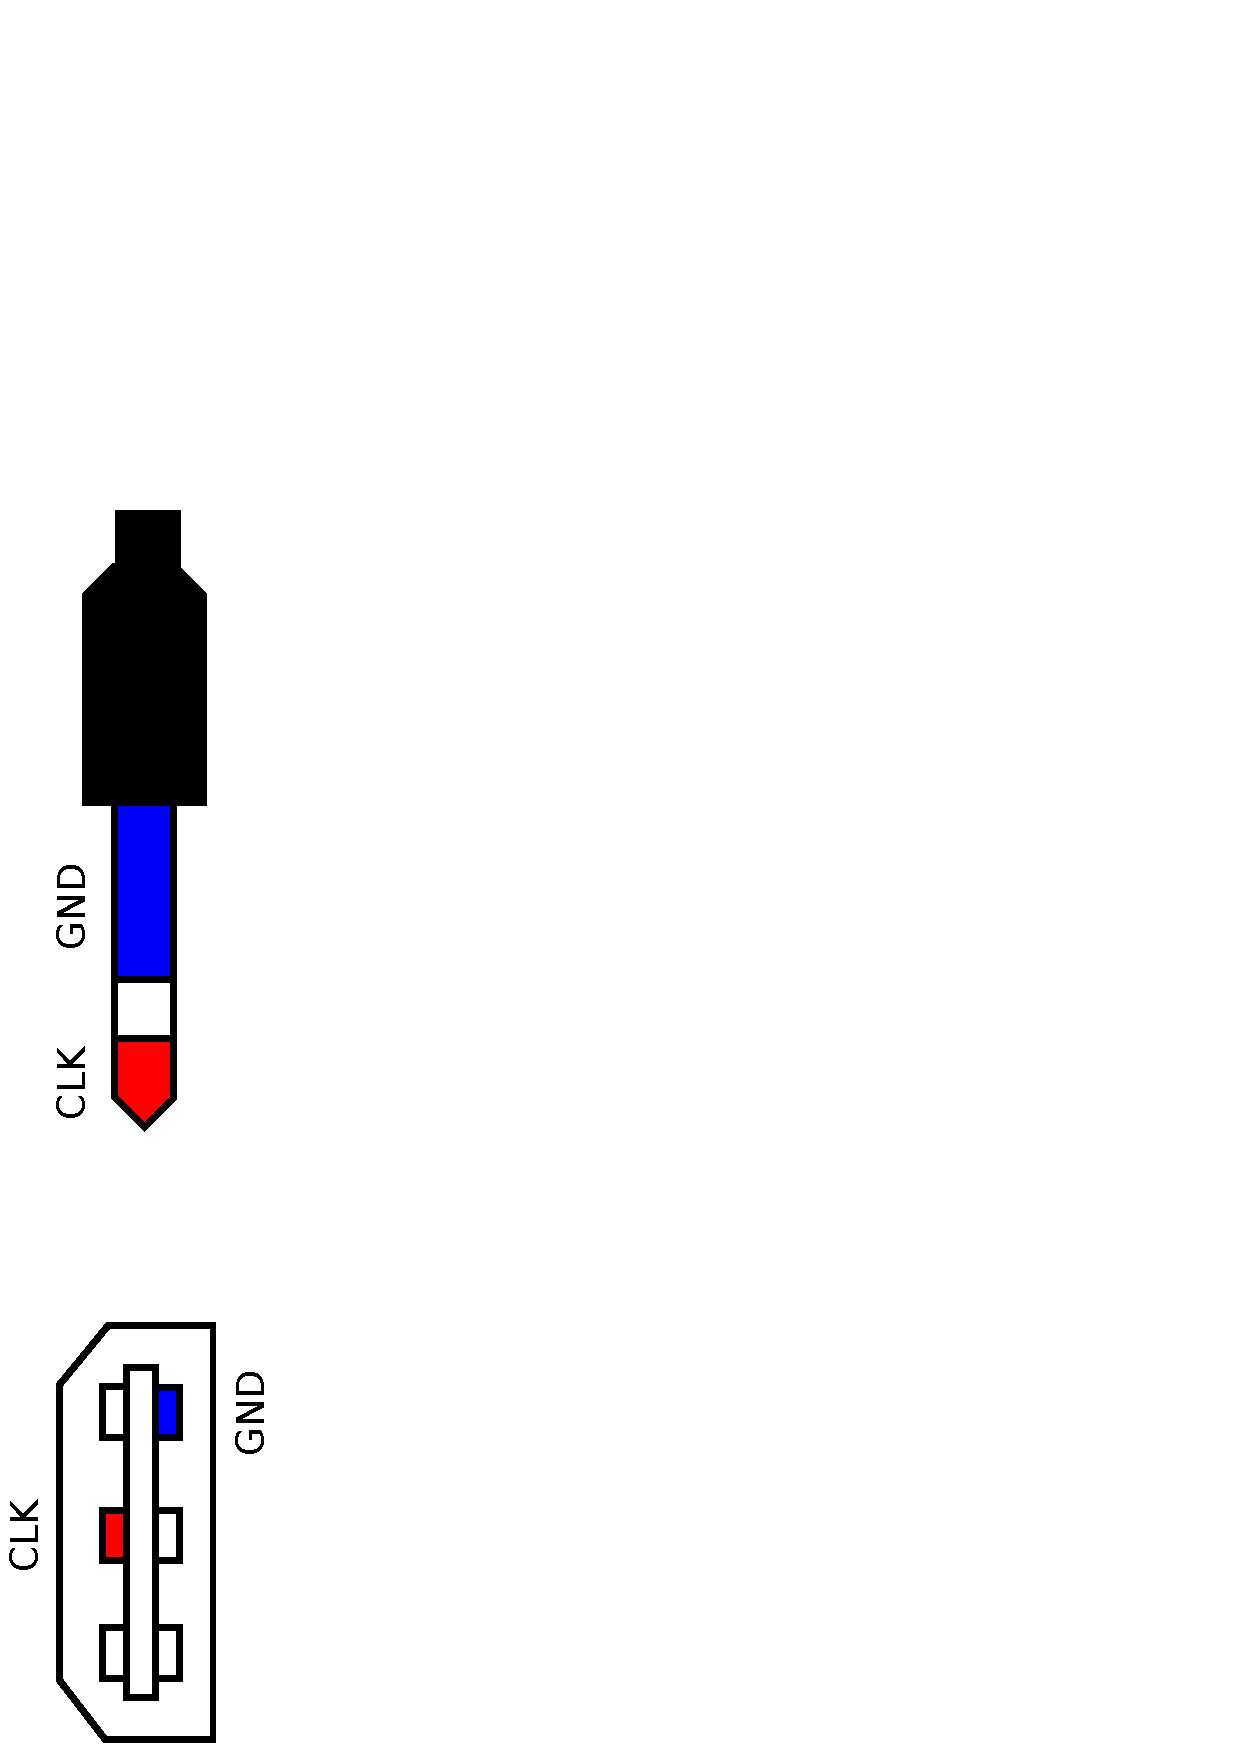
\includegraphics[clip=true,trim=0 0 460 250,angle=270,width=12cm]{analog-in}\\

As a clarification, the above diagram is looking at the cable, and the wires are probably not red and blue in reality.

Once the cable is built, connect it to the Game Boy serial port and the \textsc{sync out} of your synthesizer. In project screen, set LSDj to \textsc{analog} sync mode. The \textsc{ticks/step} setting controls how many LSDj ticks should be generated for each incoming sync signal. Depending on the synthesizer, it may be necessary to change this setting to make LSDj run at the right speed. For Korg Monotribe, it should typically be set to 6, whereas for Korg Volca, it should be C.

\section{Analog Out}

Analog Out works similar to Analog In, except that in this mode, LSDj is responsible for sending the sync signal. The cable is different than the one used for Analog In. Build it by connecting the wires as follows:

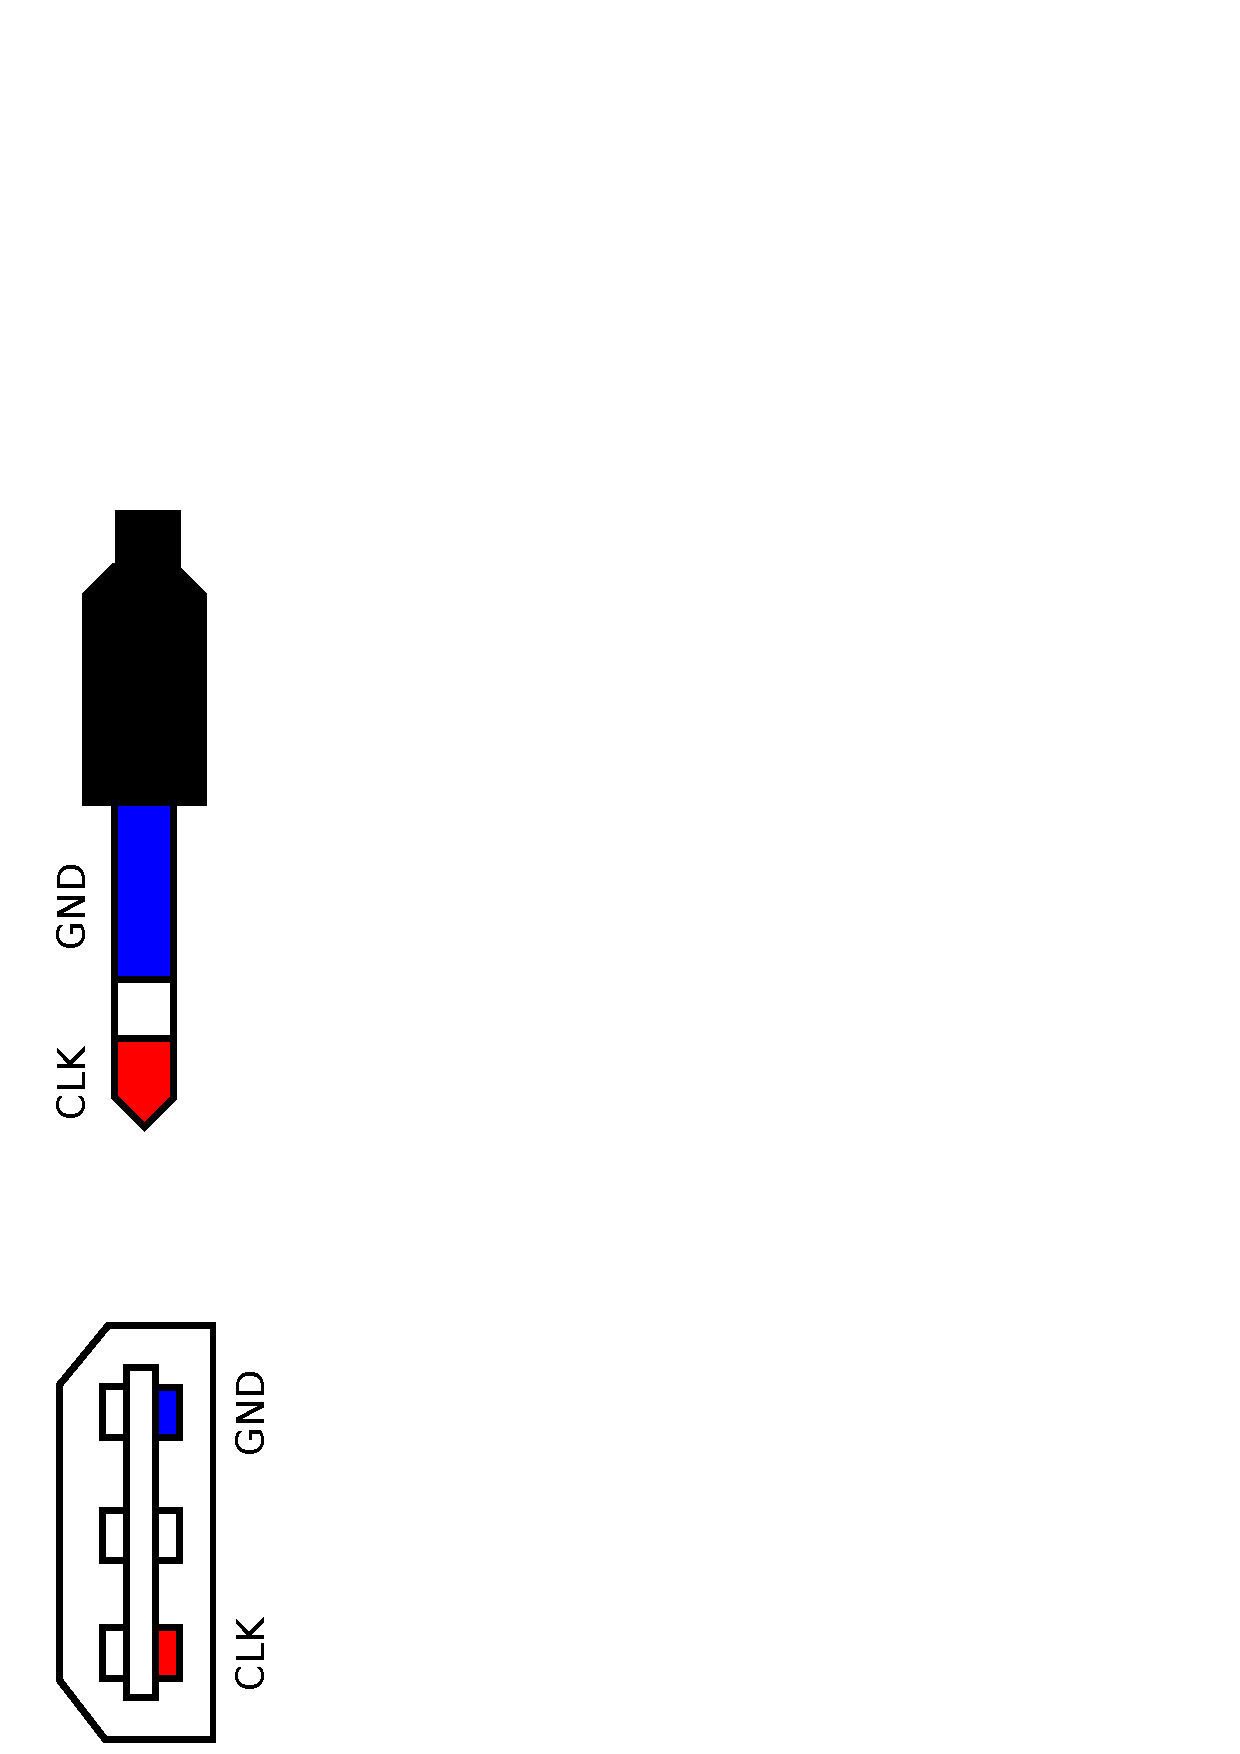
\includegraphics[clip=true,trim=0 0 460 250,angle=270,width=12cm]{analog-out}\\

As a clarification, the above diagram is looking at the cable, and the wires are probably not red and blue in reality. This cable should be connected to \textsc{sync in} of your synthesizer.

\section{Troubleshooting Cables}

When building cables, do double and triple check that the wires are connected to the right pins. You will need a multimeter for probing the pins. If they are not connected exactly like they should, you can get cables that nearly work, but the sync is a little off. The most common problem is flipped pins; remember that the diagrams are looking at the cable, not from it!

\section{Keyboard Control}

The \textsc{keybd} sync mode is not really about synchronization. Instead, it allows connecting a standard \textsc{pc} keyboard to the Game Boy, so it can be played as a piano. This is useful for live shows and improvisation. For information on how to build a \textsc{pc} keyboard to Game Boy adapter, please refer to the website at \url{http://www.littlesounddj.com}.

Important: To get a sound when playing on the keyboard, the sequencer must already be running. (Press \textsc{start} first!) The notes you play will be played back on the next step in the phrase sequencer. To get finer timing, use a faster groove for the phrase you are playing.

\subsection{Keyboard Note Layout}

\begin{figure}[htpb]
	\begin{center}
	\fbox{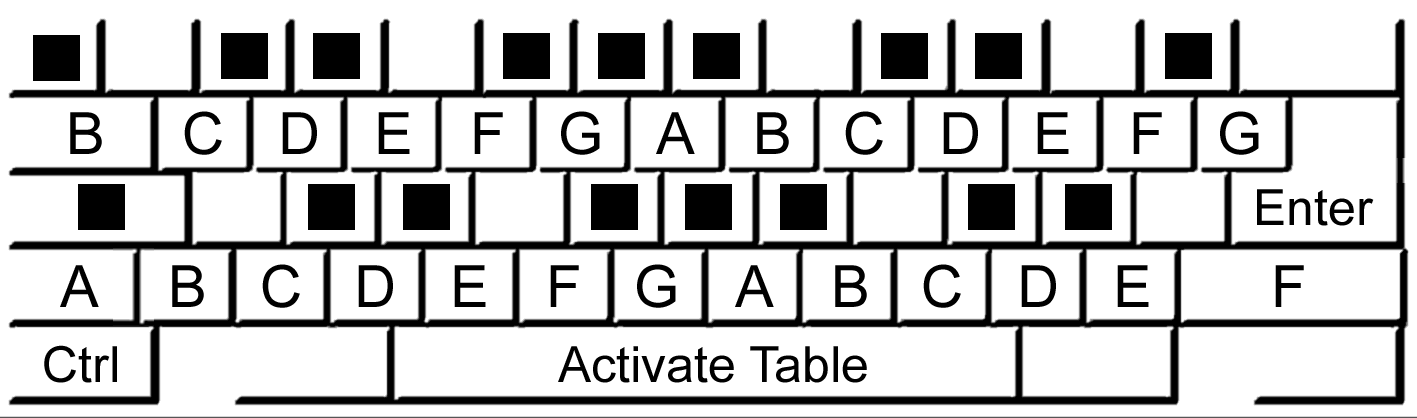
\includegraphics[width=12cm]{keybd-map}}
	\end{center}
	\caption{PC Keyboard Map}
	\label{fig:keybd-map}
\end{figure}

\begin{description}
\item[\textsc{space}] play using custom table
\item[\textsc{f1/f2}] octave down/up
\item[\textsc{f3/f4}] instrument down/up
\item[\textsc{f5/f6}] select custom table to assign to \textsc{space}
\item[\textsc{f8}] change pulse instrument playback channels (\textsc{PU1, PU2, PU1+2})
\item[\textsc{f9-f12}] toggle channel mute (switches on key press)
\item[\textsc{ctrl+(f9-f12)}] tap channel mute (switches on key press and release)
\item[\textsc{cursor}] move around cursor
\item[\textsc{enter}] play chain
\item[\textsc{ctrl+enter}] stop chain
\item[\textsc{page up/down}] \textsc{b+up/down}
\end{description}

